\documentclass[12pt]{article}

\usepackage{amsmath}
\usepackage[margin=1.25in]{geometry}
\usepackage{hyperref}
\usepackage[utf8]{inputenc}
\usepackage[english]{babel}
\usepackage{setspace}
\usepackage{indentfirst}
\usepackage{amsmath}
\usepackage{tkz-euclide}

\title{The Pertinence of PERT \\[0.25in]
  \small PERT And CPM And Why They \textit{Pert}ain to You}
\author{Nicolas Nytko}

\begin{document}
\maketitle
\newpage

\doublespacing

\section{History and Background}
When working on large-scale projects, it is important to be able to keep track of time and resources.
Project management tools, notably PERT or CPM, were developed in order to keep track of these resources and to keep track of project milestones.
Many times when working on large-scale projects, certain tasks must be done before others because they are dependent on each other, and these tasks or milestones must be done by a certain time or else the whole project must be forfeited.

Project management tools are not a modern concept, and some can be traced all the way back to ancient civilizations.  Take a look at the ancient Egyptians and how they built the \textit{Great Pyramid of Giza}.  Spanning a 20 year building period, over two million blocks of stone, each weighing about 2 tons, were dragged in and placed to build the great pyramid.  Looking at ancient records, archaeologists can infer that thousands of workers were managed by splitting them into four groups, one for each side of the pyramid.  Sophisticated planning, management, and organization was required in order to find the correct stones, then cut, move, and set them into place.

A more recent example of project management was the creation of the \textit{Gantt} chart by American mechanical engineers Henry Gantt and Frederick Taylor.
A Gantt chart is a bar chart where activities are displayed by horizontal bars, each having a length proportional to approximately how long the item should take to complete.
Gantt charts were first used in World War I in some famous projects at the time such as the Hoover Dam, and later the U.S. interstate highway network.
They are still used today because they are simple and easy to understand by the entire workforce.
However, one of the major shortcomings is that the relationships between activities and their dependencies are not shown on this chart, which is where PERT comes in.

The \textit{program evaluation and review technique}, PERT for short, is a tool used to analyze and represent the tasks and procedures needed to complete a program or project.
PERT was originally developed by the United States Navy's Special Projects Office, along with Lockheed Missile Systems in the late 1950's to help measure and estimate progress for several missile projects, the most notable of which was the \textit{UGM-27 Polaris} submarine-launched missile.
PERT was designed to manage the over 3,000 contractors employed on the \textit{Polaris} program by essentially providing a project road map that identified major milestones and how they were all dependent on each other.

One important thing to note was that the only constraint that PERT was created to deal with was time.
Since this system was developed by the U.S. Navy, one could easily deduce why other factors such as cost or quality control were not factored in.
The development of PERT was driven by a political need for the United States to compete with the Soviet Union during the cold war.
PERT was used to ensure that the Polaris project was completed during a time when the United States Government was worried about the Soviet Union's increasing stockpile of nuclear arms.
\section{How Does PERT Work?}
PERT charts are used to schedule, organize, and manage tasks and milestones in a project or program.
A PERT chart begins with one initial task or node that signifies the start of the project.
From this node, arrows are drawn to other nodes and this depicts the sequence of tasks in the project.  These tasks that are linked in order are called \textit{dependent} or \textit{serial} tasks.
Concurrent sequences of tasks can be going on at the same time, these are called \textit{parallel} or \textit{concurrent} tasks.
If a task has has multiple arrows leading to it, then all those previous tasks must be completed before that task can be done, these are considered to have \textit{task dependency}.  Nodes that have task dependency cannot be done before their dependent tasks.

Numbers are placed along the arrows to denote how much time is allotted to complete the task.
For tasks that don't take any time to complete but must be done before others, they are often depicted with a dotted arrow line.  These are called \textit{dummy activities}.
An example of a dummy activity in a software development scenario is when system files must be converted before more tasks can be completed, but relative to the project timeline the time needed to complete this task is negligible.

For each activity, three different time estimations must be defined in order to calculate the final estimation for the entire project.
The first is the \textit{optimistic time}, which is the minimum time required to accomplish an item or activity assuming that everything goes better than expected.
The second one is the \textit{pessimistic time}, which is the opposite of the optimistic time where the project is expected to go slower than usual; everything than can go wrong will go wrong in this estimation.  It is the absolute maximum amount of time something should take.
In this estimation, everything is assumed to go wrong except for major catastrophes.
The third estimation is the \textit{most likely time}, where it is the time required to go through a path assuming everything goes through normally.
From these three estimations you can find the \textit{expected time}, which accounts for the fact that some things don't always proceed normally.
This is calculated by taking a weighted average of all three previous time estimations with the likely time estimation being 4 times more heavily averaged.  This is based on an approximation of the \textit{Beta distribution}.
\[ E = \frac{T_{optimistic} + \left( 4 \times T_{likely} \right) + T_{pessimistic}}{6} \]
Along with the expected time, something called the possible variance of this estimate is also calculated.
\[ V = \frac{\left(T_{pessimistic}-T_{likely}\right)^2}{36} \]
To calculate the expected time of the full project, $E$ and $V$ are summed up for each project activity or item.
\[E_{project}=\sum_{k=1}^nE_k \quad\quad V_{project}=\sum_{k=1}^nV_k\]
The sum of every $E$ is the project expected time.  The sum of every $V$ is the variation of the entire project's expected time.  The standard deviation can then be calculated as well, it is equal to the square root of the variance, $\sqrt{V}$.

A measure of excess time and resources on a project is called the \textit{float}, or alternatively the \textit{slack}.  In a project, the amount of slack time is the amount of excess time that any particular item or activity can be delayed by and not affect subsequent tasks (free float), or affect the entire project (total float).  A project that has positive float or positive slack would indicate that the project is ahead of schedule, negative slack would indicate behind schedule, and no slack would indicate that the project is simply on schedule.
\section{Graphing With PERT}
Creating a PERT graph is not difficult, but there are some things that must be done before the graph is created.
The first is to create a task list of each thing that must be done for the project.
This list should describe things about each task, such as the approximate duration and which tasks (if any) that it is dependent on in order to be started.  Here is an example of a task list table that can be created:
\newline\newline
{\footnotesize
\begin{tabular}{|lllll|}
  \textbf{\#} & \textbf{Task} & \textbf{Length} & \textbf{Dependence} & \textbf{Type} \\
  a. & Project Planning & 1 Week & N/A & Sequential \\
  b. & Hardware Selection & 0.5 Week & a & Sequential \\
  c. & Hardware Installation & 0.5 Week & b & Sequential \\
  d. & Core Systems Programming & 4 Weeks & c & Sequential \\
  e. & Core Systems Training & 2 Weeks & d & Parallel \\
  f. & Core Systems Quality Assurance & 2 Weeks & d & Parallel
\end{tabular}}
\newline

This example table has both sequential and parallel project tasks.
This will be important when creating the PERT graph because it will be displayed as separate paths that can be taken.  It is a good idea to make this task table as detailed as possible so nothing is forgotten when the graph is created.

To draw the graph, start with the first task that does not have any task dependency.
This will be the start of your new PERT chart.
To draw the task, pick an arbitrary shape to represent tasks/nodes.  Good shapes to choose are circles, rectangles, or rounded rectangles.  Bad shapes to choose are stars, flowers, the batman symbol, or anything overly complicated.
Label this first node with a ``1'', because it is your first task.  After this first node, go down the list
in order of dependency and draw each node with its number drawn inside of it.  Once every task has been drawn,
start connecting them in order with arrows.  These arrows should be labeled with the activity name and duration.
\newline\newline
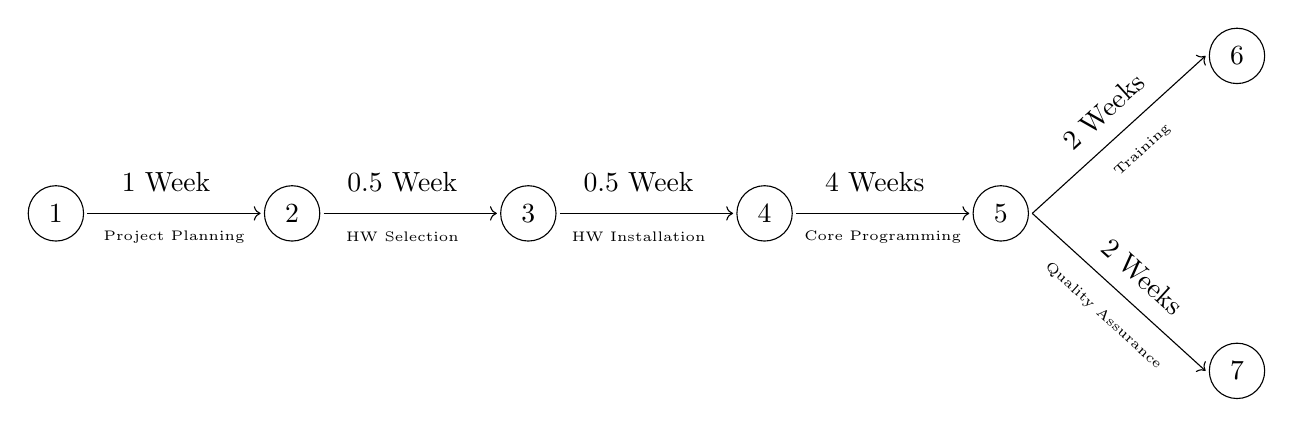
\begin{tikzpicture}
  \draw (0,0) circle(10pt);
  \node at (0,0) {1};
  \draw[->] (0.4,0) -- (2.6,0);
  \node at (1.4,0.4) {1 Week};
  \node at (1.5,-0.3) {\tiny Project Planning};
  
  \draw (3,0) circle(10pt);
  \node at (3,0) {2};
  \draw[->] (3.4,0) -- (5.6,0);
  \node at (4.4,0.4) {0.5 Week};
  \node at (4.4,-0.3) {\tiny HW Selection};
  
  \draw (6,0) circle(10pt);
  \node at (6,0) {3};
  \draw[->] (6.4,0) -- (8.6,0);
  \node at (7.4,0.4) {0.5 Week};
  \node at (7.4,-0.3) {\tiny HW Installation};
  
  \draw (9,0) circle(10pt);
  \node at (9,0) {4};
  \draw[->] (9.4,0) -- (11.6,0);
  \node at (10.4,0.4) {4 Weeks};
  \node at (10.5,-0.3) {\tiny Core Programming};
  
  \draw (12,0) circle(10pt);
  \node at (12,0) {5};
  \draw[->] (12.4,0) -- (14.6,2);
  \draw[->] (12.4,0) -- (14.6,-2);
  
  \draw (15,2) circle(10pt);
  \node at (15,2) {6};
  \node[rotate=42.27] at (13.3,1.3) {2 Weeks};
  \node[rotate=42.27] at (13.8,0.8) {\tiny Training};
  
  \draw (15,-2) circle(10pt);
  \node at (15,-2) {7};
  \node[rotate=-42.27] at (13.8,-0.8) {2 Weeks};
  \node[rotate=-42.27] at (13.3,-1.3) {\tiny Quality Assurance};
\end{tikzpicture}
\newline

The above illustration details the previously shown task chart converted into a PERT graph.  It begins with the first node, which is project planning and lasts for 1 week.  It then continues sequentially until the core programming node, where it branches into two parallel tasks.  These two tasks can be done at the same time and are not dependent on each other to be completed.

Due to its relative simplicity, PERT graphs can be created using any graphing or image editing software, though specialized programs do exist.  A quick google search shows that PERT graphing programs can range from being completely free to about \$350 USD.  For those that are more technically inclined, graphs can be created using graphing programs or markup languages such as GraphViz, TikZ/PGF, etc.  (The figure above was created with the TikZ package for LaTeX).  Or if you're desperate enough, you could even just fire up a copy of MS Paint and start drawing it by hand.
\section{CPM}
Critical Path Method, CPM, is a project management technique similar to PERT that was also developed in the 1950's.
CPM began development in 1956 by the \textit{DuPont} chemical company and computing firm \textit{Remington Rand Univac}.  The precursors to CPM, however, were originally developed and practiced by DuPont as early as 1940 and helped contribute to the success of the \textit{Manhattan Project}. 
Like PERT, it too was devised as a way to manage activity interrelationships in a project.
The Critical Path Method was named after its usage of a \textit{Critical Path}, a sequence of tasks or activities to be finished so that a project can be completed.
Items or activities on the critical path cannot be done until previous activities have been completed.

CPM was first used in 1958 to construct a new DuPont chemical plant, and then used again in 1959 to manage the shutdown of another DuPont plant.  DuPont reportedly saved about 25\% of the costs on shutdowns by using CPM by using it to efficiently plan shutdowns instead of flooding the project with labor.  CPM was dropped by DuPont once the management team responsible for it was changed.  Even though it was short-lived within DuPont, another company named Mauchly Associates started to use it.  This company helped to commercialize CPM by having it focus on scheduling efficiencies rather than cost savings.  Mauchly also conducted CPM training and transformed it into a new way of running businesses for construction companies.  However, since computer systems were still relatively expensive back in the early 1960's, CPM had a high barrier of entry for many.  It wasn't a coincidence that CPM started becoming widely popular once computers became small enough to fit on top of every office desk.

The generation of a CPM graph requires the differentiation between critical and non-critical activities.  Critical activities are identified because if any of these activities are delayed, then the whole project suffers.  The \textit{Critical Path} in CPM follows this sequence of critical activities.  The critical path is the absolutely most optimized path that goes through each critical activity and has the smallest time and resource expense.

CPM keeps track of both time and resources for each individual project item or activity.  This allows for something called \textit{project crashing}.  Let's explain it with a simple analogy: imagine you are a project manager told to finish a certain project milestone in 7 weeks, and have a budget allotment of \$10,000.  Later, you are told that the 7 weeks for the project will push back the project ship date, and must be done in 5 weeks.  With this smaller amount of time, more resources must be dedicated to the project.  Many times, this is done by modeling the increase with a simple linear relationship, however, it is up to the project manager to determine how much the resources are increased by.

While CPM and PERT sound very similar, there are some key differences to keep in mind.
When scheduling a project using, a PERT chart is created using uncertain activities, while a CPM chart is created using very well-defined activities.
When using CPM, the durations of project items are very well defined and rigid, they cannot be changed and failure to stick to those deadlines may jeopardize the entire project.
When looking at these factors, CPM can be considered to be deterministic, i.e., not accounting for any randomness or error.  Therefore, CPM only gives one time estimate.
PERT, on the other hand, is probabilistic and so gives multiple estimates: optimistic time, most likely time, and pessimistic time.  An additional difference between PERT and CPM activities is that CPM will process critical and non-critical activities differently, while PERT does not differentiate between critical and non-critical activities and all tasks are assigned the same priority.

When scheduling a project using PERT, the only factor accounted for is the time duration of each activity or item.  This is not true for CPM, which aims to minimize both the time used, but also to minimize the costs of each project item.  As stated before, this is due to the developing companies of these task methods and what their requirements were at the times.  Another interesting thing to note is that because PERT is milestone based, it is best used for projects where the activities or items are non-repetitive and do not keep showing up repeatedly.  CPM is the opposite, and is best suited for repeated activities. Because of this, PERT is more suited for research and development projects, while CPM is best suited for large-scale construction projects where the same thing may be done over and over again.
\section{PERT and CPM Today}
An example of PERT/CPM usage today is in construction projects.
Depending on the project's individual needs either PERT or CPM can be used.
(However, more often than not CPM is used).
Project times can be easily estimated based on previous knowledge and experience of other construction projects.
Most construction project milestones and events are well-defined and have a rigid time duration, making CPM an excellent candidate for project management.
For a construction project to be able to use either PERT or CPM, it must contain events that can be done independently of each other, and these events must have an order to them.
Continous processes such as several types of manufacturing or oil refining will not be able to be managed using PERT or CPM because they do not contain independent jobs to have done.

PERT is often used to schedule research and development projects.  Since in these kinds of projects the nodes are not very well defined and time durations are only approximates, PERT will work well because it does not require extremely precise numbers, nor does it require extremely rigid deadlines.  Researchers can set general project milestones given approximations for previous projects or from research and then use this to create a general time expectation for the project to be finished.  

In software development, PERT is sometimes used alongside of Agile.  Agile is a set of development principles that focuses on rapid development and feedback.  In an agile development environment, work is divided into small parts and given to cross-functional teams that work on all aspects of the iteration: planning, analysis, development, etc.  After each iteration, a working prototype is showed to shareholders or to upper management and feedback is recorded.  This allows for minimal risk and easy adaptation because each small step must be scrutinized.  In this case, PERT can be used to plan the entire project and divide it into subintervals.  Each interval is an activity on the PERT chart that takes up a duration of time, and some are dependent on others to be finished.
PERT can be used to identify which parts of the project will take the most time, and then allow project managers to optimize that item.


\section{Conclusion}
PERT is a critical tool for project management and is very commonly used nowadays for all kinds of projects.
It is very well suited for identifying key project milestones and relating them together in a specific order that maximizes project efficiency, this certain order being the critical path of the project.  Using PERT, it is very easy to get high-accuracy project duration estimates and expensive software is not necessary to calculate it.  It is simple to understand and can help efficiently manage projects and activities.  

\newpage
\begin{thebibliography}{9}
\bibitem{FederalStatisticalActivities}
  Stauber, B. Ralph et al.
  \textit{Federal Statistical Activities.}
  The American Statistician, vol. 13, no. 2, 1959, pp. 9-12. \\
  \url{www.jstor.org/stable/2682310}.
\bibitem{SearchSoftwareQuality}
  Rouse, Margaret.
  \textit{PERT chart (Program Evaluation Review Technique)}.
  SearchSoftwareQuality. WhatIs.com, May 2007. Web. 01 Dec. 2016. \\
  \url{http://searchsoftwarequality.techtarget.com/definition/PERT-chart}.
\bibitem{MindTools}
  Mind Tools.
  \textit{Critical Path Analysis and PERT Charts: Planning and Scheduling More Complex Projects.}
  Critical Path Analysis and PERT Charts. Mind Tools, n.d. Web. 01 Dec. 2016. \\
  \url{https://www.mindtools.com/critpath.html}.
\bibitem{Chron}
  Kielmas, Maria.
  \textit{History of the Critical Path Method.}
  History of the Critical Path Method. Chron, n.d. Web. 01 Dec. 2016. \\
  \url{http://smallbusiness.chron.com/history-critical-path-method-55917.html}.
\bibitem{TutorialsPoint}
  TutorialsPoint.
  \textit{PERT Estimation Technique.}
  www.tutorialspoint.com. Tutorials Point, n.d. Web. 01 Dec. 2016. \\
  \url{https://www.tutorialspoint.com/management_concepts/pert_estimation_technique.htm}.
\bibitem{KeyDifferences}
  S, Surbhi. \textit{Difference Between PERT and CPM (with Comparison Chart) - Key Differences.} Key Differences.
  Key Differences, 27 Aug. 2016. Web. 1 Dec. 2016. \\
  \url{http://keydifferences.com/difference-between-pert-and-cpm.html}.
\bibitem{azcentral}
  Berman, Craig. \textit{History of the Critical Path Method.} History of the Critical Path Method. Azcentral, n.d. Web. 1 Dec. 2016. \\
  \url{http://yourbusiness.azcentral.com/history-critical-path-method-24351.html}.
\end{thebibliography}
\end{document}
